% !TeX document-id = {e57240da-2747-4ecc-baf4-a1fe920d8231}
% Unofficial University of Cambridge Poster Template
% https://github.com/andiac/gemini-cam
% a fork of https://github.com/anishathalye/gemini
% also refer to https://github.com/k4rtik/uchicago-poster

% !TeX TXS-program:compile = txs:///latexmk -lualatex -bibtex -interaction=nonstopmode  -file-line-error

\documentclass[final]{beamer}

% ====================
% Packages
% ====================

\usepackage[T1]{fontenc}
\usepackage{lmodern}
\usepackage[orientation=portrait,size=a0,scale=1.0]{beamerposter}
\usetheme{gemini}
\usecolortheme{nott}

\usepackage{physics}
\usepackage{amsmath}
\usepackage{graphicx}
\usepackage{booktabs}
\usepackage{tikz}
\usetikzlibrary{decorations.markings,arrows.meta}
\usepackage{pgfplots}
\pgfplotsset{compat=1.14}
\usepackage{anyfontsize}
\usepackage{lipsum}
\usepackage{hyperref}
\usepackage[dvipsnames]{xcolor}

\definecolor{hanblue}{rgb}{0.27, 0.42, 0.81}
\definecolor{asparagus}{rgb}{0.53, 0.66, 0.42}
%\usepackage{xcolor}

\definecolor{coolblue}{HTML}{0072B2}   % blue
\definecolor{coolgreen}{HTML}{009E73}  % bluish-green
\definecolor{skyblue}{HTML}{56B4E9}   % Okabe-Ito sky blue
\definecolor{navy}{HTML}{2C3E70}
% ====================
% Lengths
% ====================

% If you have N columns, choose \sepwidth and \colwidth such that
% (N+1)*\sepwidth + N*\colwidth = \paperwidth
\newlength{\sepwidth}
\newlength{\colwidth}
\setlength{\sepwidth}{0.025\paperwidth}
\setlength{\colwidth}{0.45\paperwidth}

\newcommand{\separatorcolumn}{\begin{column}{\sepwidth}\end{column}}

% ====================
% Title
% ====================

\title{Scaling and cutoff effects of the topological susceptibility with gradient flow  \\in $SU(3)$ Yang--Mills theory on the lattice.}

% \author{Agajan Torayev \inst{1} \and Ben Bitdiddle \inst{2} \and Lem E. Tweakit \inst{2}}
\author{P. Butti \inst{1}, G. Catumba \inst{2}, A. Conigli \inst{3}, A. Saez \inst{4}, F. P. Panadero \inst{5}}

\institute[shortinst]{
  \inst{1} University of Southern Denmark 
  \samelineand \inst{2} Milano
  \samelineand \inst{3} Johannes Gutenberg-Universit\"{a}t Mainz 
  \samelineand \inst{4} IFIC Valencia
  \samelineand \inst{5} IFT Madrid
  }

% ====================
% Footer (optional)
% ====================

\footercontent{
  \href{https://indico.global/event/16565/contributions/161179/}{link to slides} \hfill
  % \href{https://www.example.com}{https://www.example.com} \hfill
  Lattice 2026, Maryland  \hfill
  % \href{mailto:agajan.torayev@example.com}{agajan.torayev@example.com}}
% (can be left out to remove footer)
}

% % ====================
% % Logo (optional)
% % ====================

% % use this to include logos on the left and/or right side of the header:
% \logoright{
\includegraphics[height=4cm]{logos/NCG-LOGO-INV.pdf}}
% \logoleft{
\includegraphics[height=4cm]{logos/UoN_Logo_NottinghamBlue_WhiteText_CMYK.pdf}}


% ====================
% Logos
% ====================

% Every partner logo is fitted into an identical box, so that a square emblem
% and a wide wordmark carry the same optical weight.
\newlength{\logocellw}\setlength{\logocellw}{4.6cm}
\newlength{\logocellh}\setlength{\logocellh}{1.9cm}
\newcommand{\logocell}[1]{%
  \makebox[\logocellw][c]{%
    \includegraphics[width=\logocellw,height=\logocellh,keepaspectratio]{#1}}}

% White plate: the partner logos are dark-on-transparent (or opaque white-bg)
% artwork and are illegible directly on the nottblue headline.
\newcommand{\logoplate}[1]{{\setlength{\fboxsep}{2ex}\colorbox{white}{#1}}}

% sdu.png is white artwork on transparency: it belongs on the navy, not a plate.
% \logoleft{
\includegraphics[height=4cm]{logos/sdu.png}}
\logoleft{
  \begin{tabular}{1}
    \logocell{logos/sdu.png} \\
    \logocell{logos/ific.png} \\
  \end{tabular}
}


\logoright{\logoplate{%
  \begin{tabular}[c]{@{}c@{\hspace{2ex}}c@{}}
    \logocell{logos/bicocca.png} & \logocell{logos/mainz-brutto.png} \\[2ex]
    \logocell{logos/ific.png}    & \logocell{logos/ift.png}          \\
  \end{tabular}}%
}


% ====================
% Body
% ====================


% ===== preamble additions (put near the other \usepackage lines in poster.tex) =====
\usetikzlibrary{decorations.markings,arrows.meta}

% directed link: line with an arrowhead at its midpoint
\tikzset{
  dlink/.style={
    line width=0.9pt,
    postaction={decorate},
    decoration={markings,
      mark=at position 0.58 with {\arrow{Stealth[length=2.6mm,width=2.6mm]}}}
  }
}

% \cloverleaf[scale]{a}{b}: four a-by-b rectangular leaves sharing the site x
\newcommand{\cloverleaf}[3][1]{%
\scalebox{#1}{%
\begin{tikzpicture}[x=1cm,y=1cm,baseline=(current bounding box.center)]
  \def\aa{#2}\def\bb{#3}
  \draw[dlink] (0,-\bb)--(\aa,-\bb);   \draw[dlink] (\aa,-\bb)--(\aa,0);
  \draw[dlink] (\aa,0)--(\aa,\bb);     \draw[dlink] (\aa,\bb)--(0,\bb);
  \draw[dlink] (0,\bb)--(-\aa,\bb);    \draw[dlink] (-\aa,\bb)--(-\aa,0);
  \draw[dlink] (-\aa,0)--(-\aa,-\bb);  \draw[dlink] (-\aa,-\bb)--(0,-\bb);
  \draw[dlink] (\aa,0)--(0,0);         \draw[dlink] (0,0)--(0,\bb);
  \draw[dlink] (-\aa,0)--(0,0);        \draw[dlink] (0,0)--(0,-\bb);
  \fill (0,0) circle (2pt);
  \node[font=\footnotesize] at (0.36,0.32) {$\hat\nu$};
  \node[font=\footnotesize] at (0.64,-0.20) {$\hat\mu$};
\end{tikzpicture}}%
}

\newcommand{\plaquette}[1][1]{%
\scalebox{#1}{%
\begin{tikzpicture}[x=1cm,y=1cm,baseline=(current bounding box.center)]
  \draw[dlink] (-1,-1)--(-1,1);   % bottom: x -> x+mu
  \draw[dlink] (-1,1)--(1,1);   % right:  x+mu -> x+mu+nu
  \draw[dlink] (1,1)--(1,-1);   % top:    back along -mu
  \draw[dlink] (1,-1)--(-1,-1);   % left:   down along -nu
  \fill (-1,-1) circle (1.5pt);
  \node[font=\footnotesize] at (0.01,-0.5) {$\hat\mu$};
  \node[font=\footnotesize] at (-0.28,0.5) {$\hat\nu$};
\end{tikzpicture}}%
}




\begin{document}

% Refer to https://github.com/k4rtik/uchicago-poster
% logo: https://www.cam.ac.uk/brand-resources/about-the-logo/logo-downloads
% \addtobeamertemplate{headline}{}
% {
%     \begin{tikzpicture}[remember picture,overlay]
%       \node [anchor=north west, inner sep=3cm] at ([xshift=-2.5cm,yshift=1.75cm]current page.north west)
%       {\includegraphics[height=7cm]{logos/unott-logo.eps}}; 
%     \end{tikzpicture}
% }

\begin{frame}[t]
\begin{columns}[t]
\separatorcolumn

\begin{column}{\colwidth}

  % \begin{block}{Abstract}
    The computation of the topological susceptibility in 
    lattice gauge theory requires a smoothing procedure for 
    the gluonic topological charge, with cooling and gradient 
    flow being the most commonly adopted approaches. While 
    cooling is computationally cheaper, gradient flow admits 
    a Symanzik expansion that is easier to compute and allows 
    for a clean identification of leading order cutoff effects.
    We study these effects in pure SU(3) Yang--Mills theory using 
    ensembles generated with different gauge actions at lattice 
    spacings ranging from 0.04 fm to 0.12 fm. By combining different 
    levels of improvement for the flow kernel with several discretisations 
    of the topological charge operator, we study the contributions 
    to lattice artefacts arising from the action, flow, and observable,
    aiming to disentangle their respective effects. We present 
    preliminary results on the scaling of the topological susceptibility
    and the effectiveness of improvement strategies.
\end{block}
%
  
% \begin{equation}
%     \clover[0.6]{2}{1}
% \end{equation}

\lipsum[1]
\lipsum[1]

  % Requires xcolor (loaded automatically by beamer).
\colorlet{jbl}{blue!65!black}
\colorlet{jgr}{green!40!black}
\colorlet{jre}{red!70!black}

\begin{block}{A fully $\mathcal{O}(a^2)$-improved susceptibility}

  In the Symanzik effective theory, the susceptibility measured at flow
  time $t_c$ admits the expansion~\cite{Ramos:2015baa,RamosMartinez:2023tvx}
  \begin{equation*}
    \boxed{
    \expval{\chi}_\text{latt} = \expval{\chi_0}
    + a^2\qty[
        {\color{jbl} \expval{\chi_2}} +
        {\color{jgr} \expval{\chi S_{2,c}}} + 
        {\color{jre} \expval{\chi S_{2,\text{fl}}}}
    ]
    + \order{a^4} \,,
    }
  \end{equation*}
  where the $\langle \cdot \rangle$ on the r.h.s. are computed in the continuum theory. Each $\mathcal{O}(a^2)$ insertion has a distinct origin --- and a
  distinct cure:

  \begin{itemize}
    \item \textcolor{jbl}{\textbf{Observable:}}
          $\textcolor{obsC}{\langle\chi_2\rangle}$ comes from the \emph{classical} $\mathcal{O}(a^{2})$ expansion of the observable, in our case the topological charge : $\chi_{latt} = \chi_{0} + a^{2}\chi_{2} + ...$
          \vspace{2mm}

          $\;\Rightarrow\;$ Can be made zero using $\hat q^{\mathrm{imp}} $ $\to $ use \textbf{improved observables!}
          \vspace{2mm}
    \item \textcolor{jgr}{\textbf{Action:}}
      $\textcolor{actC}{\langle\chi\,S_{2,c}\rangle}$ is the insertion of the
      $\mathcal{O}(a^2)$ counterterms of the path-integral action,
      \begin{equation*}
        S_\text{conf} = \frac{\beta}{3}\sum_x\qty(
            c_0\sum_{\mu<\nu} \mathrm{Re} \tr \qty(1 - \vcenter{\hbox{\plaquette[0.7]}})
        +   c_1\sum_{\mu<\nu} \mathrm{Re} \tr \qty(1 - \vcenter{\hbox{\cloverleaf[0.7]{2}{1}}})
        ).
      \end{equation*}

      $\;\Rightarrow\;$ \emph{use \textbf{improved actions!}}
    \item \textcolor{jre}{\textbf{Flow:}}
      $\textcolor{floC}{\langle\chi\,S_{2,\mathrm{fl}}\rangle}$ originates
          from the flow-kernel action. By using
          \vspace{2mm}
          \begin{equation*}
            \partial_t V_\mu(x,t) = -g_0^2\,
            \Big(1+\frac{a^2}{12}\,\nabla_\mu^{\ast}\nabla_\mu\Big)\,
            \big[\partial_{x,\mu} S^{\mathrm{LW}}(V_t)\big]\, V_\mu(x,t)\, ,
          \end{equation*}
  \end{itemize}

  it vanishes $S_{2,\mathrm{fl}} = 0$ $\;\Rightarrow\;$ \emph{use the \textbf{Zeuthen flow!}~\cite{Ramos:2015baa}}

  % The residual term, proportional to the flow-time derivative of $\chi$ at
  % $t_c$, tracks the $\mathcal{O}(a^2)$ ambiguity of the flow scale and is
  % measured directly from the $t$-dependence. Combining all three yields a
  % fully $\mathcal{O}(a^2)$-improved determination of $\chi$.
\end{block}


  \begin{block}{Datasets}
    The ensembles are generated with HMC using \href{https://igit.ific.uv.es/alramos/latticegpu.jl}{\verb|LatticeGPU.jl|}   
    package \cite{???}, running on GPUs.
    \begin{description}
        \item[\textbf{Big volumes~\cite{RamosMartinez:2023tvx}:}]
        {\color{asparagus}
            Big volumes ($L\simeq 2.6\text{--}5.7\,\mathrm{fm}$), modest statistics. \\
            4 different gauge actions + Zeuthen flow + clover $\hat Q$ (not improved).
        } 
        \item[\textbf{Fully improved:}] 
        {\color{hanblue}
            Fixed volume ($L\simeq 1.4\,\mathrm{fm}$), bigger statistics. \\ 
            Luscher-Weisz action + Zeuthen and Wilson flow + improved $\hat Q$ 
            (clover + rectangle).
        }
    \end{description}
    % The ensembles are generated with standard HMC with \verb|LatticeGPU.jl| package \cite{???}, running on GPUs.
    \medskip
    \centering
    \begin{minipage}[t]{0.48\textwidth}
        \centering
        \setlength{\tabcolsep}{0.55em}
        \renewcommand{\arraystretch}{1.05}
        \begin{tabular}{lcccc}
        \toprule
            action & $\beta$ & $a\,[\mathrm{fm}]$ & $L/a$ & $N_\mathrm{conf}/\tau_\mathrm{int}$\\
        \midrule
            W   & {\color{asparagus} 6.13  } & {\color{asparagus} 0.076 }  & {\color{asparagus} 64    } & {\color{asparagus} 328   }  \\
                & {\color{asparagus} 6.25  } & {\color{asparagus} 0.063 }  & {\color{asparagus} 64    } & {\color{asparagus} 224   }  \\
                & {\color{asparagus} 6.2929} & {\color{asparagus} 0.060 }  & {\color{asparagus} 64    } & {\color{asparagus} 114   }  \\
                & {\color{asparagus} 6.35  } & {\color{asparagus} 0.055 }  & {\color{asparagus} 64    } & {\color{asparagus} 104   }  \\
                & {\color{asparagus} 6.42  } & {\color{asparagus} 0.050 }  & {\color{asparagus} 64    } & {\color{asparagus} 149   }  \\
                & {\color{asparagus} 6.52  } & {\color{asparagus} 0.043 }  & {\color{asparagus} 64    } & {\color{asparagus} 152   }  \\
        \midrule
            IW  & {\color{asparagus} 2.79  }  & {\color{asparagus} 0.074 }   & {\color{asparagus} 64    } & {\color{asparagus} 92    } \\
                & {\color{asparagus} 2.91  }  & {\color{asparagus} 0.062 }   & {\color{asparagus} 64    } & {\color{asparagus} 25    } \\
                & {\color{asparagus} 2.945 }  & {\color{asparagus} 0.060 }   & {\color{asparagus} 64    } & {\color{asparagus} 24    } \\
                & {\color{asparagus} 3.00  }  & {\color{asparagus} 0.055 }   & {\color{asparagus} 64    } & {\color{asparagus} 43    } \\
                & {\color{asparagus} 3.11  }  & {\color{asparagus} 0.048 }   & {\color{asparagus} 64    } & {\color{asparagus} 25    } \\
                & {\color{asparagus} 3.18  }  & {\color{asparagus} 0.044 }   & {\color{asparagus} 64    } & {\color{asparagus} 23    } \\
        \midrule
            DBW2 & {\color{asparagus} 1.111 } & {\color{asparagus} 0.076 }        & {\color{asparagus} 64    }    & {\color{asparagus} 23    }     \\
                 & {\color{asparagus} 1.16  } & {\color{asparagus} 0.069 }        & {\color{asparagus} 64    }    & {\color{asparagus} 22    }     \\
                 & {\color{asparagus} 1.24  } & {\color{asparagus} 0.059 }        & {\color{asparagus} 64    }    & {\color{asparagus} 24    }     \\
                 & {\color{asparagus} 1.30  } & {\color{asparagus} 0.052 }        & {\color{asparagus} 64    }    & {\color{asparagus} 21    }     \\
                 & {\color{asparagus} 1.35  } & {\color{asparagus} 0.048 }        & {\color{asparagus} 64    }    & {\color{asparagus} 357   }     \\
                 & {\color{asparagus} 1.40  } & {\color{asparagus} 0.043 }        & {\color{asparagus} 64    }    & {\color{asparagus} 24    }     \\
        \bottomrule
        \end{tabular}
    \end{minipage}\hfill
    \begin{minipage}[t]{0.48\textwidth}
        \centering
        \setlength{\tabcolsep}{0.55em}
        \renewcommand{\arraystretch}{1.05}
        \begin{tabular}{lcccc}
        \toprule
        action & $\beta$ & $a\,[\mathrm{fm}]$ & $L/a$ & $N_\mathrm{conf}/\tau_\mathrm{int}$\\
        \midrule
        LW  & {\color{asparagus} 4.45 }  & {\color{asparagus} 0.091} & {\color{asparagus} 64   } & {\color{asparagus} 209  }  \\
            & {\color{asparagus} 4.59 }  & {\color{asparagus} 0.075} & {\color{asparagus} 64   } & {\color{asparagus} 157  }  \\
            & {\color{asparagus} 4.71 }  & {\color{asparagus} 0.064} & {\color{asparagus} 64   } & {\color{asparagus} 117  }  \\
            & {\color{asparagus} 4.76 }  & {\color{asparagus} 0.060} & {\color{asparagus} 64   } & {\color{asparagus} 89   }  \\
            & {\color{asparagus} 4.83 }  & {\color{asparagus} 0.054} & {\color{asparagus} 64   } & {\color{asparagus} 84   }  \\
            & {\color{asparagus} 4.93 }  & {\color{asparagus} 0.048} & {\color{asparagus} 64   } & {\color{asparagus} 77   }  \\
            & {\color{asparagus} 5.00 }  & {\color{asparagus} 0.044} & {\color{asparagus} 64   } & {\color{asparagus} 62   }  \\
        \midrule
        LW  & {\color{hanblue} 4.2703} & {\color{hanblue} 0.12  } & {\color{hanblue} 12    }& {\color{hanblue} ---   } \\
            & {\color{hanblue} 4.2703} & {\color{hanblue} 0.12  } & {\color{hanblue} 16    }& {\color{hanblue} ---   } \\
            & {\color{hanblue} 4.4464} & {\color{hanblue} 0.09  } & {\color{hanblue} 16    }& {\color{hanblue} ---   } \\
            & {\color{hanblue} 4.6178} & {\color{hanblue} 0.07  } & {\color{hanblue} 20    }& {\color{hanblue} ---   } \\
            & {\color{hanblue} 4.7594} & {\color{hanblue} 0.06  } & {\color{hanblue} 24    }& {\color{hanblue} ---   } \\
            & {\color{hanblue} 4.8739} & {\color{hanblue} 0.05  } & {\color{hanblue} 28    }& {\color{hanblue} ---   } \\
        \bottomrule
        \end{tabular}

        \medskip
        \justifying
    \end{minipage}

    {\small W: Wilson plaquette; IW: Iwasaki; LW: L\"uscher--Weisz
    tree-level Symanzik; DBW2}

\end{block}



\end{column}

\separatorcolumn

\begin{column}{\colwidth}

  \begin{block}{Continuum limit}
    We compute $\chi$ in units of the flow scale $t_0$, and we attempt a continuum limit.
    \begin{figure}
      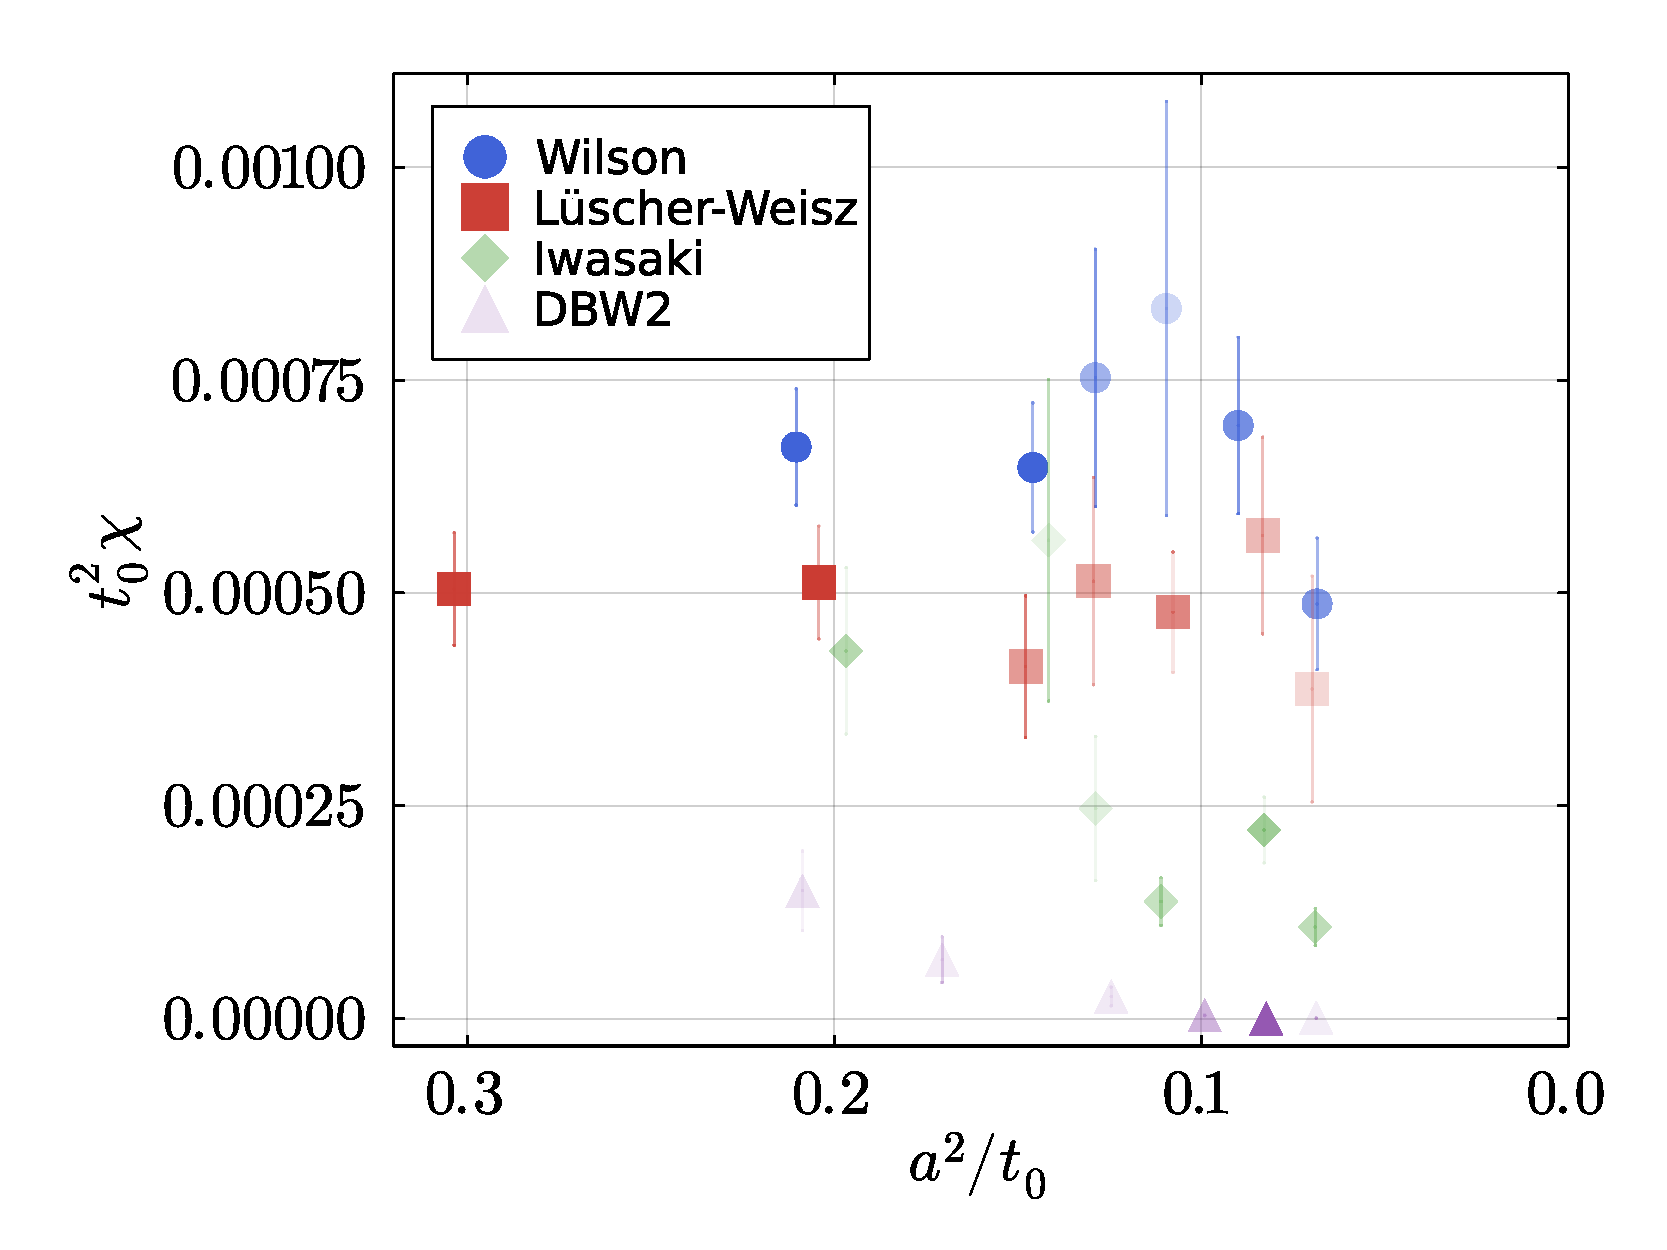
\includegraphics[scale=0.6]{PLOTS/L64_CL.pdf}
      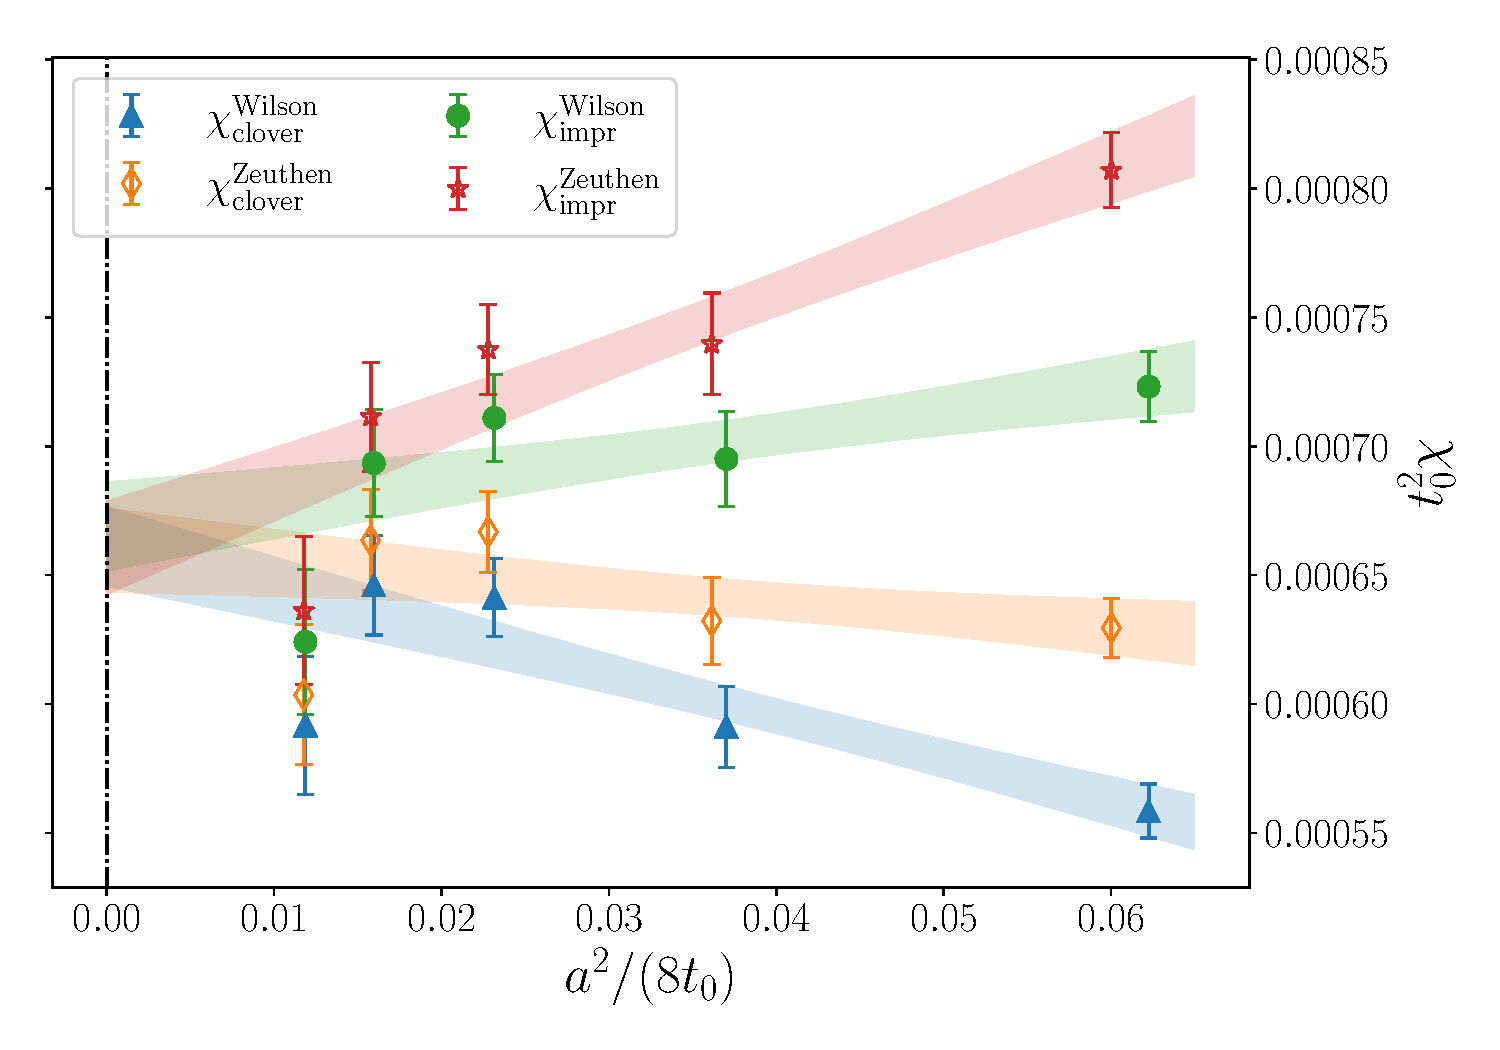
\includegraphics[scale=0.7]{PLOTS/cl_behaviour_t0.pdf}
    \end{figure}
    \begin{description}
        \item[\textbf{Left:}] The Iwasaki and DBW2 ensembles are effectively frozen — topology is suppressed and the charge is badly undersampled — so we attempt a continuum extrapolation only for Wilson and Lüscher-Weisz, whose limits agree.
        \item[\textbf{Right:}] 4 extrapolations from a single set of Lüscher-Weisz configurations with more statistics, spanning all combinations of Wilson/Zeuthen flow and clover/improved charge. The four definitions differ only at $\order{a^2}$ and, despite slopes of opposite sign, converge to a common continuum value — a nontrivial consistency check on the charge and flow discretisations.
    \end{description}
\end{block}

  \colorlet{jbl}{blue!65!black}
\colorlet{jgr}{green!40!black}
\colorlet{jre}{red!70!black}

\begin{block}{Cutoff effects at $\order{a^2}$}
  The higher-statistics LW ensembles let us dissect the Symanzik expansion term by
  term, comparing $\chi$ from Zeuthen versus Wilson flow and from the clover versus
  the improved charge.

  Ratios of definitions measured on the \emph{same} configurations cancel
  $\langle {\chi}_\text{cont} \rangle$ together with the action term $\langle{\chi S_{2,c}}\rangle$.
  Zeuthen flow further sets $\langle{\chi S_{2,\text{fl}}}\rangle = 0$, and the improved
  charge $\langle{\chi_2^\text{impr}}\rangle = 0$, leaving a single term in each ratio:
  %
  \begin{align*}
    {\chi^\text{Zeuthen}_\text{clover}}/{\chi^\text{Zeuthen}_\text{impr}}
      &= 1 + a^2\,{\color{jbl} \expval{\chi_2^\text{clover}}} + \order{a^4} \,, \\[0.4em]
    {\chi^\text{Wilson}_\text{impr}}/{\chi^\text{Zeuthen}_\text{impr}}
      &= 1 + a^2\,{\color{jre} \expval{\chi S_{2,\text{fl}}^{W}}} + \order{a^4} \,.
  \end{align*}
  %
  The two contributions are thus accessible separately from our data.
  \skipline
  %
  \begin{figure}
    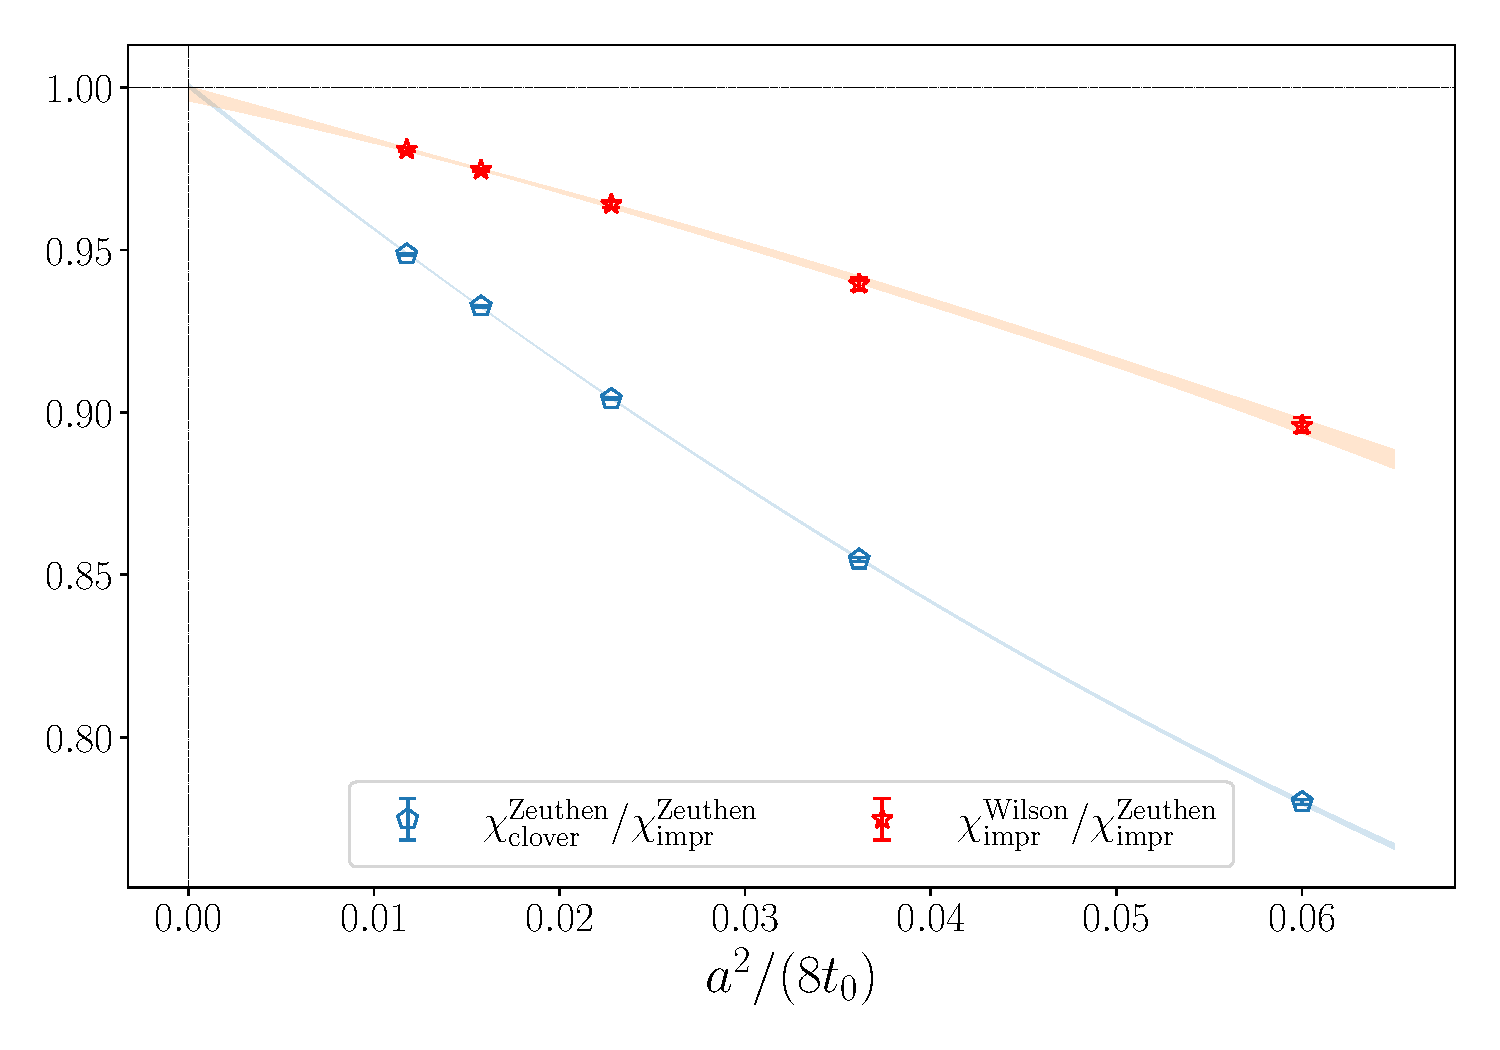
\includegraphics[scale=1.]{PLOTS/ratios_cutoff_cl.pdf}
  \end{figure}
  %
  The blue and red points isolate cutoff effects from the charge discretisation and the flow, respectively
   A quadratic dependence on $a^2$ describes the full range up to $a^2/t_0 = 0.48$,
  while a linear fit already suffices when restricted to the finest lattices. The $a^3$ contribution is therefore a small 
  but  genuine correction rather than an over-fitting artefact.

  Both ratios approach unity as $a^2 \to 0$ by construction. They quantify only \emph{classical} cutoff effects, which are cancelled exactly by combining Zeuthen flow  with the improved charge. \emph{Quantum} cutoff effects instead originate from the action used to generate the gauge configurations. The continuum-limit analysis in the left panel is designed to probe these effects, but with the present statistics and the unimproved clover charge they remain hidden within the statistical uncertainty. We plan to resolve them using Wilson-action ensembles covering the same lattice-spacing range with comparable statistics.
\end{block}
  
  
  \begin{block}{Outlook}
  	\begin{itemize}
  		\item \textbf{Generate matched Wilson-action ensembles} over the same lattice-spacing range and with comparable statistics, to resolve the action-induced \textbf{quantum cutoff effects}
  		\medskip
  		\item \textbf{Compare the approach to the continuum} across the available gauge actions, flow kernels, and charge discretisations, testing improvement and universality
  		\medskip
  		\item \textbf{Perform a combined continuum extrapolation} of the compatible determinations, quantify the remaining systematic uncertainties, and compare the resulting precision with state-of-the-art calculations.
  	\end{itemize}
  \end{block}

  \begin{block}{References}
    % \lipsum[1]

    \nocite{*}
    \footnotesize{\bibliographystyle{plain}\bibliography{poster}}

  \end{block}

\end{column}
\separatorcolumn
\end{columns}


\begin{figure}
  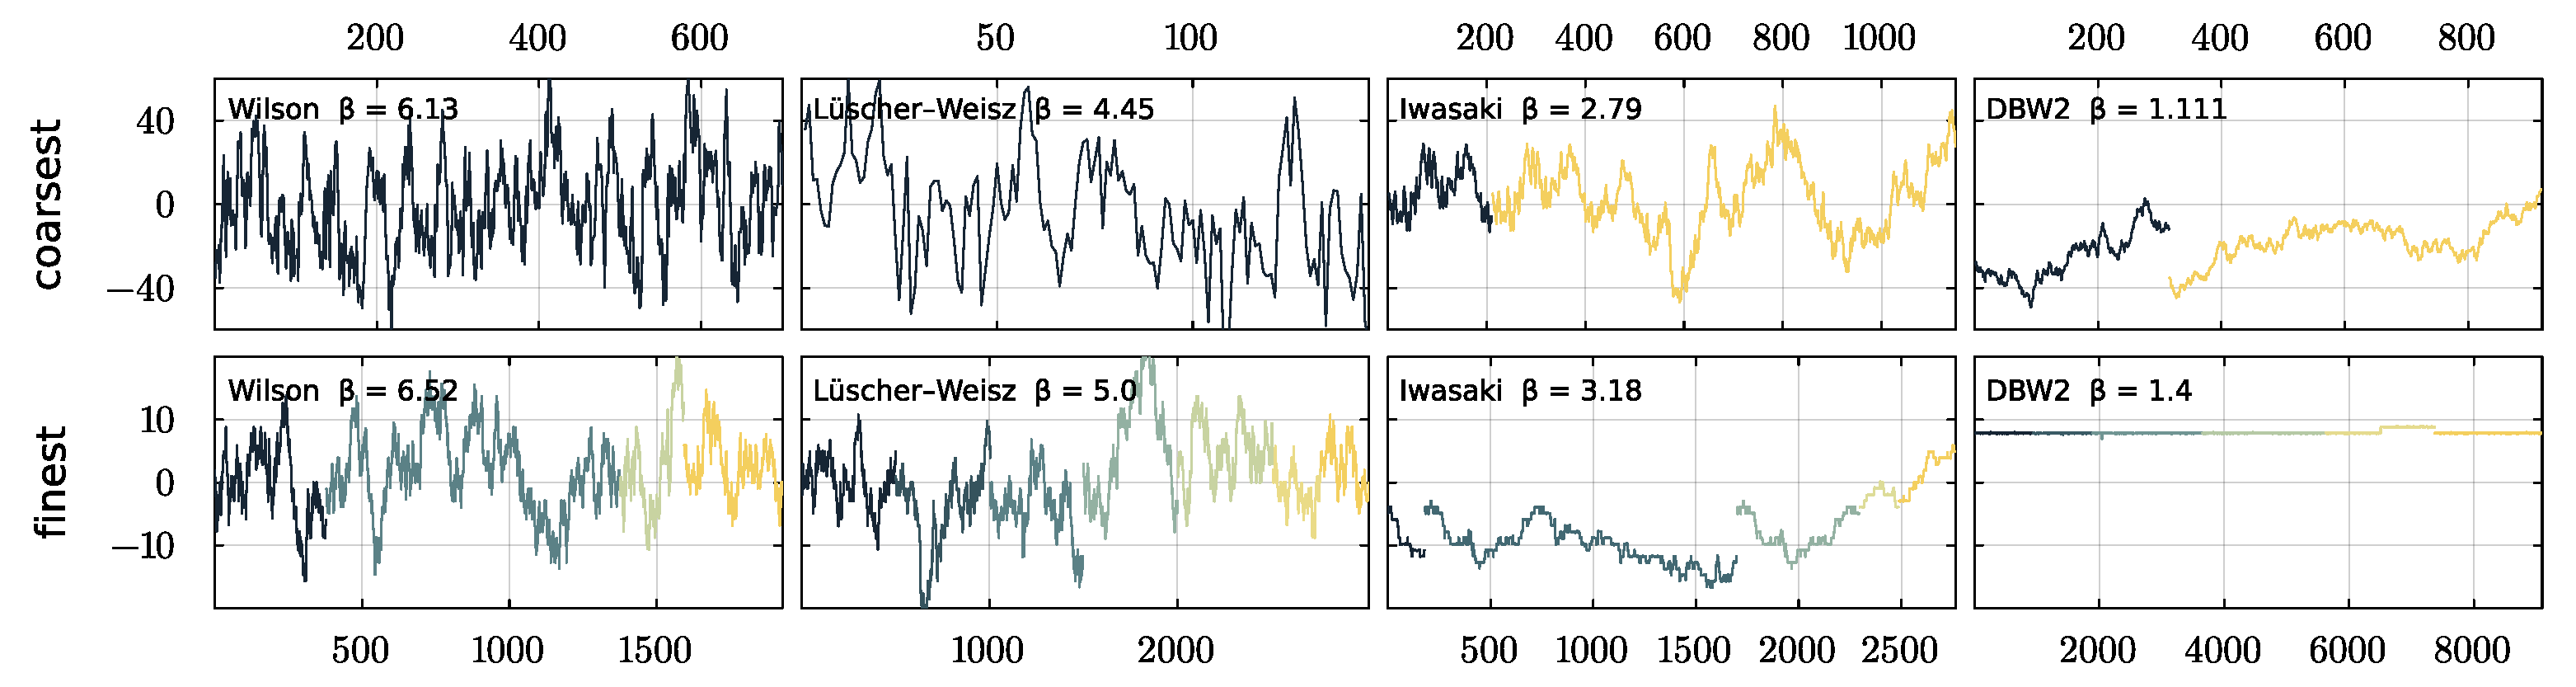
\includegraphics[scale=1.]{PLOTS/histories.pdf}
\end{figure}
\end{frame}

\end{document}
